% !TEX encoding = UTF-8 Unicode
% ------------------------------------------------------------------------------
% Este fichero es parte de la plantilla LaTeX para la realización de Proyectos
% Final de Grado, protegido bajo los términos de la licencia GFDL.
% Para más información, la licencia completa viene incluida en el
% fichero fdl-1.3.tex

% Copyright (C) 2012 SPI-FM. Universidad de Cádiz
% ------------------------------------------------------------------------------

A lo largo de este capítulo se detallará la arquitectura general del sistema de información, el diseño fí­sico de datos, el diseño detallado de componentes software y el diseño de la interfaz de usuario:

\section{Arquitectura del Sistema}

En esta sección se define la arquitectura general del sistema de información, especificando la infraestructura tecnológica necesaria para dar soporte al software y la estructura de los componentes que lo forman.


\subsection{Arquitectura Fí­sica} \label{sec:arquitectura-fisica}

El desarrollo de este proyecto no precisa de ningún elemento hardware adicional al equipo de trabajo del alumno. Se ha utilizado un portátil MacBook Pro de 15 pulgadas, con procesador Intel Core i7 de 2.2 GHz y 16GB de memoria RAM DDR3. Para la realización de pruebas, se usará tanto este equipo como otro portátil del propio alumno, donde se instalará todo el software requerido para comprobar que la instalación y ejecución de la aplicación responde adecuadamente en un equipo diferente. En este caso será un portátil Acer con procesador Dual Core, 4GB de memoria RAM y disco duro SSD. \\

Respecto al software, el MacBook trabaja bajo el sistema operativo macOS Sierra. Todo el proyecto se ha desarrollado utilizando el IDE NetBeans 8.0.2 y usando el servidor de aplicaciones GlassFish en un entorno local. Para la documentación, se ha utilizado TeXShop, como herramienta de edición para \LaTeX. Para las pruebas, el portátil a utilizar correrá bajo Windows 7, usando el mismo IDE y servidor de aplicaciones. \\

Respecto al entorno de producción, la aplicación web se alojará en un servidor que se contratará para tal fin. Por lo tanto, solo se requerirá acceso al servidor para la instalación de, en este caso, el servidor de aplicaciones Wildfly (JBoss) -habiendo sido probado previamente en entorno local de desarrollo-, siendo este similar a GlassFish, por lo que la aplicación apenas requerirá cambio alguno y aportará algo más de robustez y calidad. Los usuarios del sistema podrán hacer uso del mismo utilizando cualquier dispositivo con acceso a internet a través de un navegador web, como sus propios móviles, tablets o PCs. \\

En el apartado \ref{sec:entorno-construcción} se describirá detalladamente todo el software, lenguaje, frameworks, etc. utilizados para el desarrollo del sistema.


\subsection{Arquitectura Lógica} \label{sec:arquitectura-logica}

Para el desarrollo de esta aplicación web se ha utilizado una arquitectura de 3 capas, basada en el patrón de diseño Modelo-Vista-Controlador (MVC), donde la primera capa correspondería a la capa de usuario, la segunda la de negocio y por último la capa de datos.

\vspace{10mm}

\begin{figure}[H]
\centering
  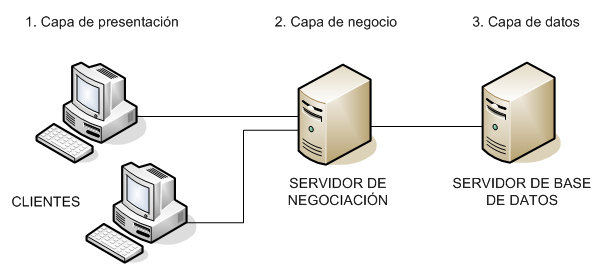
\includegraphics[scale=.55]{img/arquitectura-tres-capas.jpg}
  \caption{Representación de Arquitectura de 3 Capas}
  \label{fig:arquitectura-tres-capas}
\end{figure}

\vspace{10mm}

La programación por capas es un modelo de desarrollo software en el que el objetivo primordial es la separación (desacomplamiento) de las partes que componen un sistema software o también una arquitectura cliente-servidor: lógica de negocios, capa de presentación y capa de datos. De esta forma, por ejemplo, es sencillo y mantenible crear diferentes interfaces sobre un mismos sistema sin requerirse cambio alguno en la capa de datos o lógica.\\

La ventaja principal de este estilo es que el desarrollo se puede llevar a cabo en varios niveles y, en caso de que sobrevenga algún cambio, solo afectará al nivel requerido sin tener que revisar entre el código fuente de otros módulos (\cite{bib:wikipedia-programacion-por-capas}).

\paragraph*{Capa de presentación (frontend)}

Este grupo de artefactos software conforman la capa de presentación del sistema, incluyendo tanto los componentes de la vista como los elementos de control de la misma. \\

Es la capa que ve el usuario, denominada también \textit{capa de usuario}. Presenta el sistema al usuario, le comunica la información y captura la información del usuario en un mínimo de proceso (realiza un filtrado previo para comprobar que no hay errores de formato). También es conocida como interfaz gráfica y debe tener la característica de ser amigable (entendible y fácil de usar) para el usuario. Esta capa se comunica únicamente con la capa de negocio.

\paragraph*{Capa de negocio}

Esta capa recibe las peticiones del usuario y se envían las respuestas tras el proceso. Se denomina capa de negocio (o de lógica del negocio) porque es aquí donde se establecen todas las reglas que deben cumplirse. Esta capa se comunica con la capa de presentación, para recibir las solicitudes y presentar los resultados, y con la capa de datos, para solicitar al gestor de base de datos almacenar o recuperar datos de él. 

\paragraph*{Capa de persistencia}

Este grupo de artefactos software conforman la capa de integración del sistema, incluyendo las clases de abstracción para el acceso a datos.\\

Es donde residen los datos y es la encargada de acceder a los mismos. Está formada por un gestor de base de datos que realiza todo el almacenamiento de datos, recibe solicitudes de almacenamiento o recuperación de información desde la capa de negocio.\\

Es común que a la capa de negocio y de datos de los sistemas web se denomine conjuntamente como backend de la aplicación.\\

Como se ha comentado anteriormente, el patrón de diseño usado para el desarrollo del proyecto ha sido Modelo-Vista-Controlador, el cual separa los datos y la lógica de negocio de una aplicación de la interfaz de usuario y el módulo encargado de gestionar los eventos y las comunicaciones. Para ello MVC propone la construcción de tres componentes distintos que son el modelo, la vista y el controlador, es decir, por un lado define componentes para la representación de la información, y por otro lado para la interacción del usuario.​ Este patrón de arquitectura de software se basa en las ideas de reutilización de código y la separación de conceptos, características que buscan facilitar la tarea de desarrollo de aplicaciones y su posterior mantenimiento (\cite{bib:wikipedia-modelo-vista-controlador}).

\vspace{10mm}

\begin{figure}[H]
\centering
  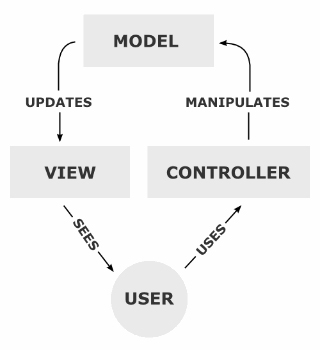
\includegraphics[scale=.55]{img/proceso-MVC.jpg}
  \caption{Proceso del Patrón MVC}
  \label{fig:proceso-MVC}
\end{figure}

\vspace{10mm}

\paragraph*{Modelo}

Es la representación de la información con la cual el sistema opera, por lo tanto gestiona todos los accesos a dicha información, tanto consultas como actualizaciones, implementando también los privilegios de acceso que se hayan descrito en las especificaciones de la aplicación (lógica de negocio). Envía a la \textit{vista} aquella parte de la información que en cada momento se le solicita para que sea mostrada al usuario. Las peticiones de acceso o manipulación de información llegan al \textit{modelo} a través del \textit{controlador}.

\paragraph*{Controlador}

Responde a eventos (acciones del usuario) e invoca peticiones al \textit{modelo} cuando se hace alguna solicitud sobre la información (por ejemplo, editar un documento o un registro en la base de datos). También puede enviar comandos a su \textit{vista} asociada si se solicita un cambio en la forma en que se presenta el \textit{modelo} (por ejemplo, desplazamiento o scroll por un documento o por los diferentes registros de una base de datos), por tanto se podría decir que el \textit{controlador} hace de intermediario entre la \textit{vista}  y el \textit{modelo}.

\paragraph*{Vista}

Presenta el \textit{modelo} (información y lógica de negocio) en un formato adecuado para interactuar (la interfaz de usuario), por tanto requiere de dicho \textit{modelo} la información que debe representar como salida.\\

Por tanto, aunque la arquitectura de 3 capas o niveles y el patrón MVC presenten sus similitudes y diferencias, cada uno tiene su función y son compatibles entre sí, de ahí el uso de ambos en el presente proyecto. A continuación, se presenta una gráfica comparativa de ambos modelos. 

\vspace{10mm}

\begin{figure}[H]
\centering
  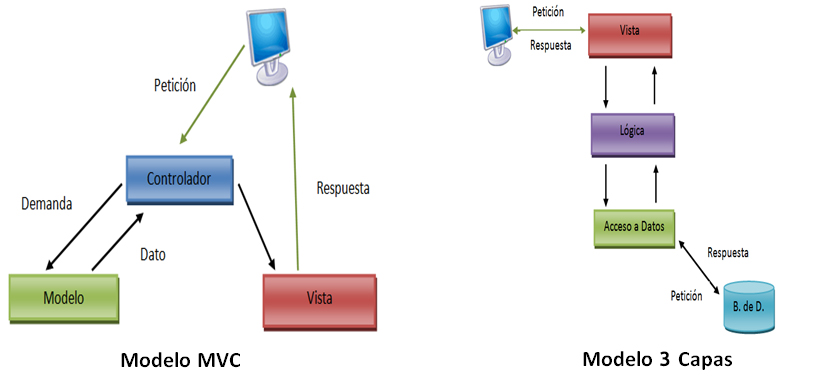
\includegraphics[scale=.50]{img/MVC-vs-3-capas.jpg}
  \caption{Comparativa entre modelo MVC y arquitectura de 3 capas}
  \label{fig:MVC-vs-3-capas}
\end{figure}

\vspace{10mm}


\section{Diseño Fí­sico de Datos}

Habiendo realizado previamente el modelo de conceptual de clases, detallado en la sección \ref{sec:modelo-conceptual}, se puede tener una idea de la estructura física que tendrá los datos en el sistema de gestión de base de datos (SGBD) a utilizar, en este caso PostgreSQL, teniendo en cuenta que aparecerán nuevas tablas en la BD provenientes de las relaciones entre las clases. Pero, por supuesto, hay que tener en cuenta que el acceso a los mismos se realice de una forma eficaz e independiente al resto de la implementación.\\ 

Y es por ello por lo que la arquitectura lógica del sistema se divide en 3 capas bien diferenciadas. La tercera de las capas contendrá el DAO (\textit{Data Access Object, Objeto de Acceso a Datos}), encargado del acceso a los datos físicos y única capa que realizará cambios en los mismos. Esto permite que si aflora la necesidad de cambios en la estructura de nuestros datos, o incluso cambiar de SGBD, las demás capas queden totalmente al margen de estos cambios, siendo un trámite independiente sin afectar -dependiendo del cambio, claro está- a la lógica de negocio o la interfaz de usuario. 


\section{Diseño de la Interfaz de Usuario} 

A continuación se muestra un prototipo de la interfaz de usuario del sistema para PC. Se mostrarán las páginas principales de la aplicación web de manera generalizada: pantalla de registro de usuario, inicio de sesión, pantalla generalizada de la aplicación una vez iniciada la sesión y página con prototipo de tabla de datos (para listado de usuarios, servicios, clases, etc.). 


\vspace{10mm}

\begin{figure}[H]
\centering
  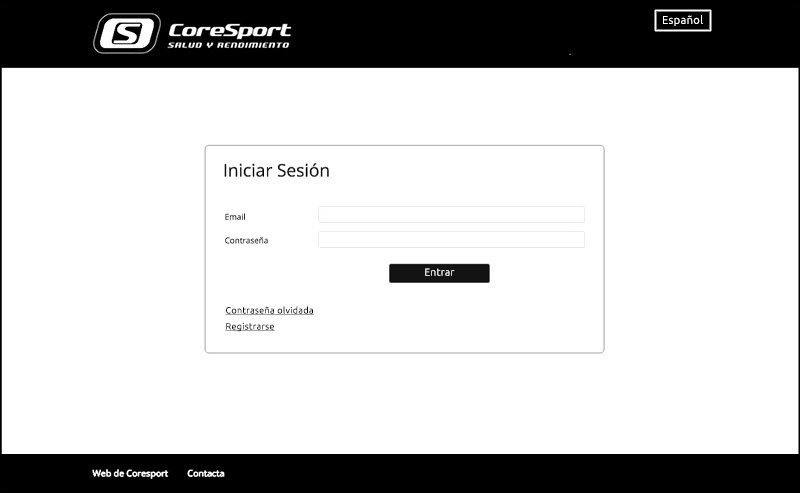
\includegraphics[scale=.40]{img/interfaz/inicio-sesion.jpg}
  \caption{Interfaz de usuario: Inicio de sesión}
  \label{fig:interfaz-inicio-sesion}
\end{figure}

\begin{figure}[H]
\centering
  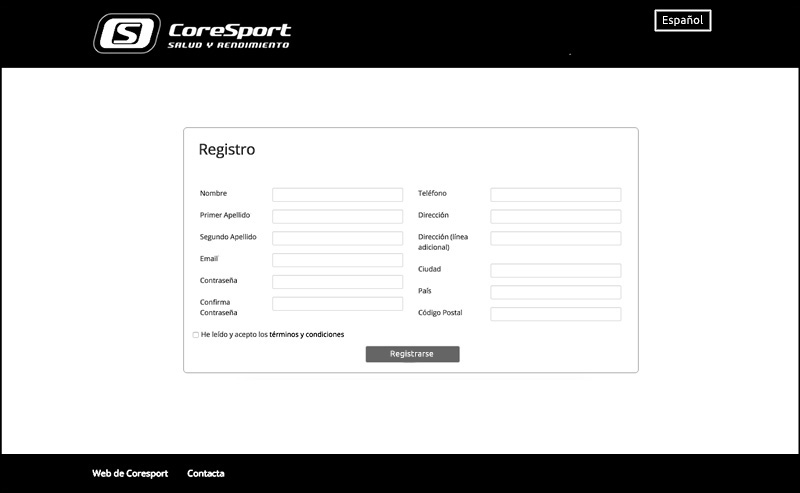
\includegraphics[scale=.40]{img/interfaz/registro.jpg}
  \caption{Interfaz de usuario: Registro}
  \label{fig:interfaz-registro}
\end{figure}

\begin{figure}[H]
\centering
  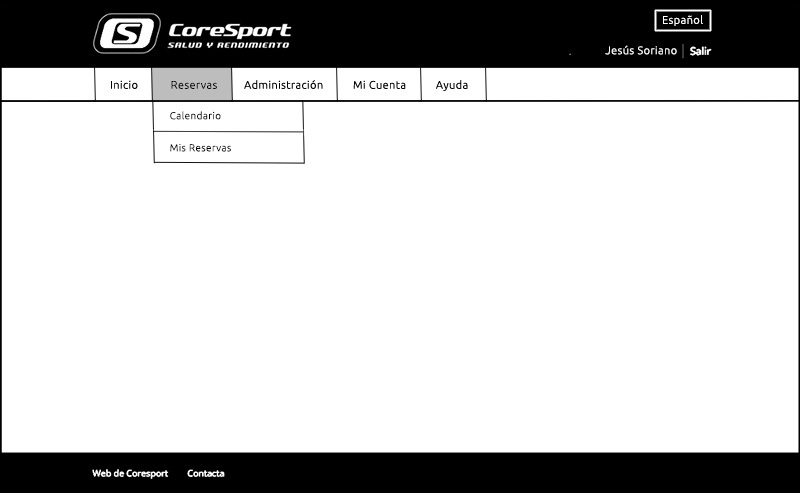
\includegraphics[scale=.40]{img/interfaz/pantalla-principal.jpg}
  \caption{Interfaz de usuario: Pantalla general}
  \label{fig:interfaz-pantalla-principal}
\end{figure}

\begin{figure}[H]
\centering
  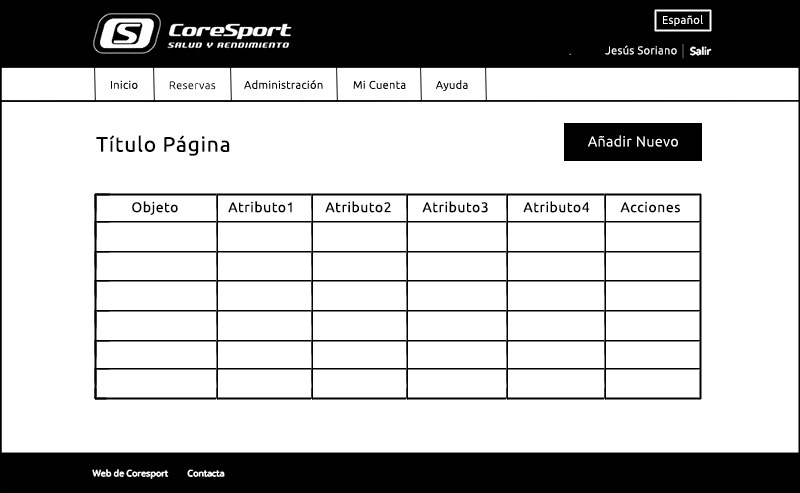
\includegraphics[scale=.40]{img/interfaz/cuadro-general.jpg}
  \caption{Interfaz de usuario: Pantalla con tabla de datos}
  \label{fig:interfaz-cuadro-general}
\end{figure}


Asimismo, se ha realizado el diseño de las pantallas para dispositivos de menor tamaño, al ser un diseño adaptativo dependiendo del mismo. A continuación se podrán visualizar los mockups realizados para la interfaz de dispositivos móviles. En este caso, las pantalla de inicio de sesión, pantalla general de usuario y menú desplegado.


\begin{figure}[H]
\centering
  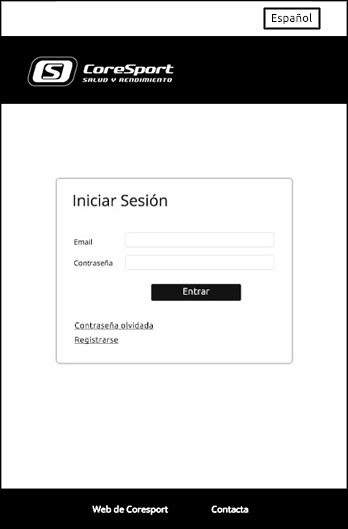
\includegraphics[scale=.50]{img/interfaz/inicio-sesion-movil.jpg}
  \caption{Interfaz de usuario para dispositivos móviles: Inicio de sesión}
  \label{fig:interfaz-inicio-sesion-movil}
\end{figure}

\begin{figure}[H]
\centering
  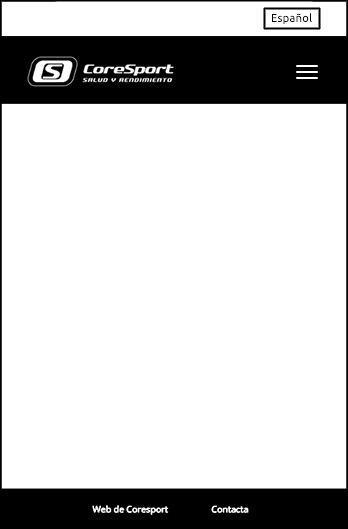
\includegraphics[scale=.50]{img/interfaz/pantalla-principal-movil.jpg}
  \caption{Interfaz de usuario para dispositivos móviles: Pantalla general}
  \label{fig:interfaz-pantalla-principal-movil}
\end{figure}

\begin{figure}[H]
\centering
  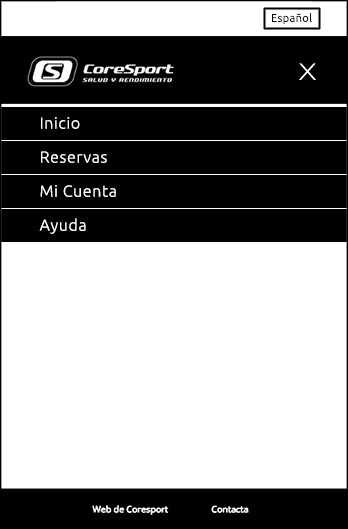
\includegraphics[scale=.50]{img/interfaz/menu-movil.jpg}
  \caption{Interfaz de usuario para dispositivos móviles: Menú desplegable}
  \label{fig:interfaz-menu-movil}
\end{figure}


Además, la figura \ref{fig:interfaz-navegacion} muestra el diagrama de navegación entre pantallas. Observamos que es una navegación sencilla; la página que se mostraría al acceder a la aplicación sería la de inicio de sesión. Si se trata de un usuario registrado, podrá acceder directamente a la página principal de la aplicación (\textit{Home}) a través del usuario y contraseña. En caso contrario, habría que navegar a la página de registro para que, una vez registrado, pueda acceder al sistema llegando a la página principal mencionada. Desde esta página de inicio (\textit{Home}) se podrá navegar, a través del menú y/o enlaces disponibles, hasta las distintas vistas de la interfaz. En todo momento será posible cerrar la sesión del usuario, volviendo a la página de inicio de sesión, o cambiar el idioma de la interfaz mediante la opción destinada a ello en la parte superior derecha de la pantalla. \\ 

En el diagrama observamos que se navega hacia la vista de una tabla de datos. Este es un ejemplo de tantas vistas como hay en el sistema. Algunos ejemplos de tablas de datos pueden ser las página donde se listan los servicios, clases, citas, usuarios (para administradores) o reservas del usuario. Existen muchas más páginas en el sistema para navegar, como las páginas de perfil, cambio de contraseña, bandeja de entrada, calendario, creación/edición de servicios/clases/citas/usuarios para administradores, etc. \\

Esta navegación ocurrirá de la misma manera en todo tipo de dispositivos, donde el único cambio sería el diseño de la pantalla, como hemos observado en los prototipos para PC y móvil.


\begin{figure}[H]
\centering
  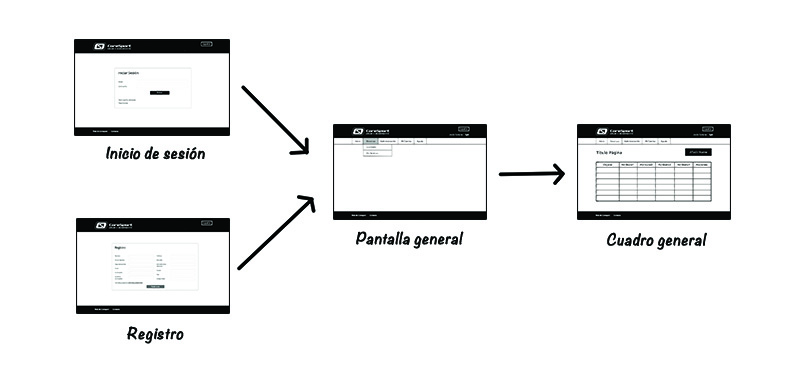
\includegraphics[scale=.50]{img/interfaz/navegacion.jpg}
  \caption{Interfaz de usuario: Diagrama de navegación}
  \label{fig:interfaz-navegacion}
\end{figure}

